\documentclass[10pt]{article}

\usepackage{amsmath}

\newcommand{\myvec}[1]{\ensuremath{\begin{pmatrix}#1\end{pmatrix}}}

\newcommand{\mydet}[1]{\ensuremath{\begin{vmatrix}#1\end{vmatrix}}}

\newcommand{\solution}{\noindent \textbf{Solution: }}

\providecommand{\brak}[1]{\ensuremath{\left(#1\right)}}

\providecommand{\norm}[1]{\left\lVert#1\right\rVert}
\usepackage{graphicx}
\usepackage{float}

\let\vec\mathbf

\title{Coordinate Geometry}
\author{Saipreet Pattjoshi (spattjoshi@sriprakashschools.com)}

\begin{document}
\maketitle
\section*{10$^{th}$ Maths - Chapter 7}
This is Problem-4 from Exercise 7.2
\begin{enumerate}
\item  Find the ratio in which the line segment joining the points (-3, 10) and (6, – 8) is divided by (-1, 6).  \\
\solution \\
Given Data:\\
\begin{align}
           \vec{A} = \myvec{-3\\10}\\
           \vec{B} = \myvec{6\\-8}\\
           \vec{C} = \myvec{-1\\6}\\
           \end{align}
To find: ratio dividing them\\
Now, 
\begin{align}
\vec{C} = \frac{\vec{A}+n\vec{B}}{n+1}\\
\vec{C} = \frac{1}{1+n} \times \myvec{\myvec{-3\\10}+n\times \myvec{6\\-8}}\\
= \frac{1}{1+n} \times \myvec{-3+6n\\10-8n}
\end{align}
By taking x
\begin{align}
-1= \frac{-3+6n}{1+n}\\
\implies -3+6n=-1-n\\
\implies 6n+n =-1+3\\
 \implies 7n=2\\
 \implies n=\frac{2}{7}
\end{align}	
now, by taking y 
\begin{align}
6= \frac{10-8n}{n+1}\\
\implies 10-8n=6+6n\\
\implies 10-6=6n+8n\\
\implies 4=14n\\
\implies n=\frac{2}{7}
\end{align}
Therefore,the ratio which divides A and B is 2:7.\\
\end{enumerate}

\begin{figure}[H]
			\centering
			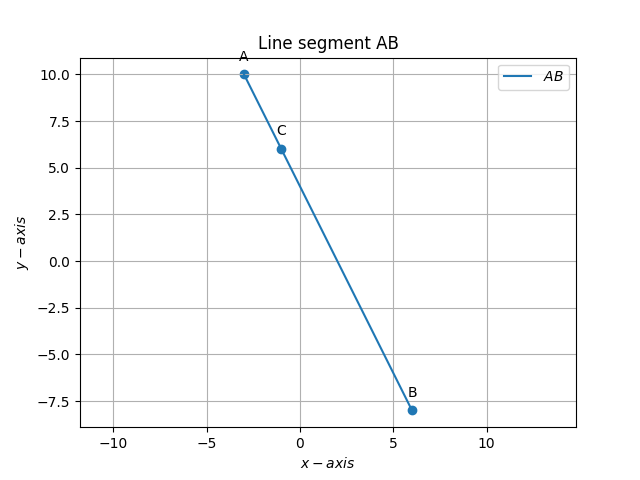
\includegraphics[width=\columnwidth]{figs/Figure_1.png}
			\caption{Line segment AB}
			\label{fig:6}
		\end{figure}
\end{document}
